% ===================================================================
%  Αρχείο: 15437_tikz.tex (Fragment)
%  Αυτόματη μετατροπή μέσω doc2latex.py & TikZ conversion
% ===================================================================

ΘΕΜΑ 2

Δίνεται η συνάρτηση $f$, της οποίας η γραφική παράσταση φαίνεται στο

παρακάτω σχήμα:

\begin{center}
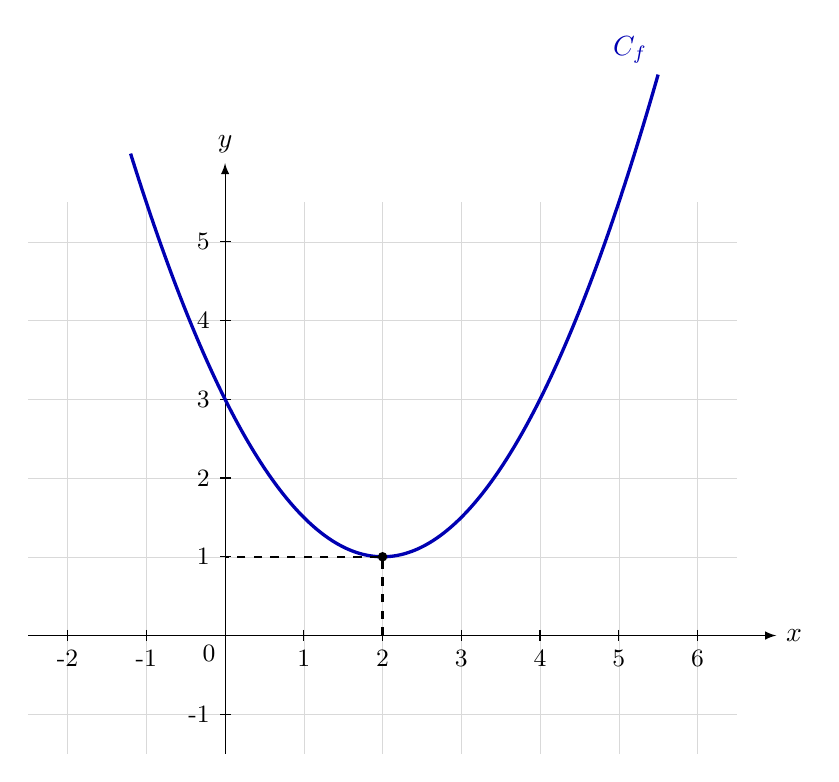
\begin{tikzpicture}[scale=1, >=latex]
    \draw[very thin, color=gray!30] (-2.5,-1.5) grid (6.5,5.5);
    \draw[->] (-2.5,0) -- (7,0) node[right] {$x$};
    \draw[->] (0,-1.5) -- (0,6) node[above] {$y$};
    
    \foreach \x in {-2,-1,1,2,3,4,5,6}
        \draw (\x,2pt) -- (\x,-2pt) node[below, font=\small] {\x};
    \foreach \y in {-1,1,2,3,4,5}
        \draw (2pt,\y) -- (-2pt,\y) node[left, font=\small] {\y};
    \node[below left, font=\small] at (0,0) {$0$};
    
    % Function with min at (2,1)
    % f(x) = 1 + (x-2)^2 / 3  or similar
    \draw[very thick, color=blue!70!black, samples=100, smooth, domain=-1.2:5.5] plot (\x, {1 + (\x-2)*(\x-2)*0.5}) node[above left] {$C_f$};
    
    % Highlight minimum
    \draw[dashed, thick] (2,0) -- (2,1) -- (0,1);
    \filldraw (2,1) circle (1.5pt);
\end{tikzpicture}
\end{center}

\begin{alist}
\item Να βρείτε το πεδίο ορισμού της συνάρτησης.

\monades{7}

\item Να προσδιορίσετε το ολικό ελάχιστο της συνάρτησης, καθώς και τη θέση αυτού.

\monades{8}

\item Να βρείτε τα διαστήματα στα οποία η συνάρτηση είναι

\begin{rlist}
\item γνησίως φθίνουσα
\item γνησίως αύξουσα
\end{rlist}

\monades{10}
\end{alist}
